% !Mode:: "TeX:UTF-8"%确保文档utf-8编码
%commands:
%environments:  
\documentclass[xetex,compress]{mybeamer}
%8pt, 9pt, 10pt, 11pt, 12pt, 14pt, 17pt, 20pt
%draft – no graphics, footlines,...
%handout – no overlays
%xcolor=x11names – define more names for colors
%,aspectratio=169


\usetheme{Singapore}
\usecolortheme{rose}
%albatross fly crane seagull beetle wolverine dove beaver
% innercolortheme lily orchid rose               the colors of blocks. 
%outer color theme whale seahorse dolphin          headline, footline, and sidebar




\title{改性Bi{\scriptsize 2}O{\scriptsize 3}基光催化剂的制备\\[10pt]及其光催化性能研究}
%\subtitle
%\date
%\institute
%\logo
\author{答辩人:万泽}
\institute{指导教师:李建章 教授}
\logo{
\includegraphics[scale=0.2]{figures/四川理工学院图标.jpg}}
\date{2013年12月19日}

\begin{document}

\begin{frame}
\titlepage
\end{frame}
%plain  for large firgure  , fragile   can catcode ,mainly for verbatim environment


\begin{frame}
\frametitle{目录}
\setcounter{tocdepth}{1}
\tableofcontents[pausesections]%pausesections section pause
\end{frame}


\section{前言}%beamer class divided into section subsection subsubsection
%section* etc add to navigation bars not the toc
\subsection{引言}
\begin{frame}
\frametitle{引言}
\begin{block}{}
太阳能是唯一可再生的碳中性能源,取之不尽用之不竭,是化石能源的良好替代品。直接利用太阳能作为清洁能源是二十一世纪科学界的重大挑战。尤其在目前能源短缺和环境污染问题日益严重的背景下,不管是直接利用太阳能分解水制备氢气还是直接利用太阳能参与某些化学反应等都具有非常重要的意义。
\end{block}
\end{frame}


\subsection{光催化机理}
\begin{frame}
\frametitle{光催化机理}
\begin{columns}
\column{0.5\textwidth}
\begin{block}{}
\centering
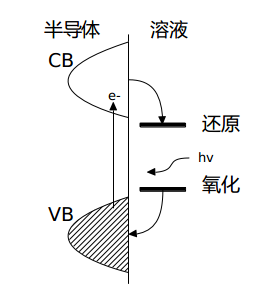
\includegraphics[scale=0.6]{figures/光催化机理图} 
\end{block}
\column{0.5\textwidth}
\begin{block}{}
半导体有一个禁带能宽,当照射进来的光的能量超过禁带能宽时,就会把价带(VB)的电子激发并进入导带(CB)。这样在价带会形成空穴,而在导带会形成额外的电子,通常这些空穴—电子对是成对出现的。
\end{block}
\end{columns}
\end{frame}



\begin{frame}
\frametitle{Fujishima的开创性工作}
\begin{block}{}
\centering
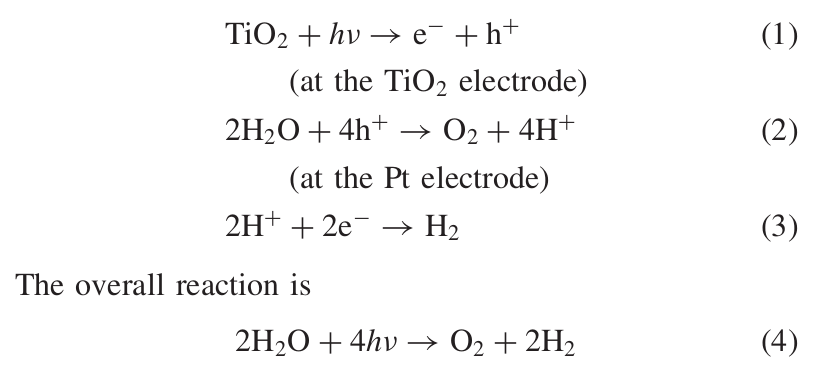
\includegraphics[scale=0.3]{figures/光分解水化学反应式} 
\end{block}
\begin{block}{}
其中TiO2是光电阳极释放电子,Pt是光电阴极在这里释放氧气。整个反应就是水的分解反应。这个光化学电池量子效率是非常低下的,大约为0.1。
\end{block}
\end{frame}

\subsection{纳米三氧化二铋的性质}
\begin{frame}
\frametitle{纳米三氧化二铋的性质}
\begin{columns}
\column{0.7\textwidth}
\begin{block}{}
\centering
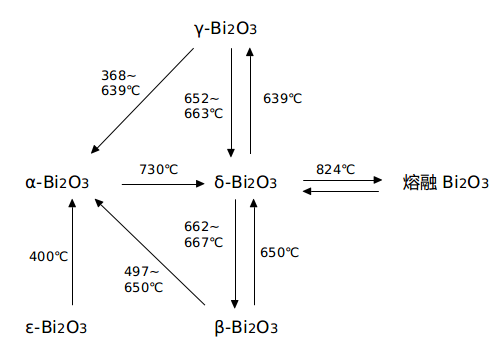
\includegraphics[width=\linewidth]{figures/Bi2O3转变温度} 
\end{block}
\column{0.3\textwidth}
\begin{block}{}
其中α-Bi2O3是室温下最稳定的构型,α-Bi2O3的禁带能宽为2.85 eV,对大部分可见光都应有吸收和响应。
\end{block}
\end{columns}
\end{frame}

\begin{frame}
\frametitle{三氧化二铋的缺陷}
\begin{columns}
\column{0.5\textwidth}
\begin{block}{光生电子—空穴复合率过高}
其中光生电子—空穴对复合率过高主要是通过调整光催化材料的晶体结构,比如通过提高结晶度加速光生电子—空穴对的分离,或者更细小的纳米粒子也会促进光生电子和空穴的分离。
\end{block}
\column{0.5\textwidth}
\begin{block}{结构不太稳定}
而Bi2O3结构不太稳定的问题Lei Huang做了专门的探讨。α-Bi2O3在空气中存放6个月就会部分转变成Bi2O2CO3,这一过程在水溶液中会进一步加速进行,这可能是因为空气中的CO2溶于水生成HCO3-和α-Bi2O3发生了反应。
\end{block}
\end{columns}
\end{frame}


\subsection{掺杂改性理论}
\begin{frame}
\frametitle{掺杂改性理论}
\begin{block}{}
金属掺杂目前认为主要有两点:一是引入杂化轨道从而降低禁带能宽,二是过渡金属可能捕捉电子从而降低光生电子─空穴复合率。非金属掺杂理论目前还没有形成一致的见解,有以下三种说法:一是非金属掺杂同样降低了禁带能宽,二是引入不纯的能级,三是比如N掺杂引入了额外的氧空位。
\end{block}
\end{frame}

\subsection{异质结改性理论}
\begin{frame}
\frametitle{异质结改性理论}
\begin{block}{}
构建物质的异质结有时能够达到比单独两个物质更好的光催化活性。这是因为两个不同物质的CB(导带)和VB(价带)能级差异,使得光生电子能够在两个物质融合的晶格面发生小能级的跃迁,从而将一次大的能级跃迁变成几次能级更小的跃迁。而多个能级晶格面的存在还提高了光生电子─空穴对分离率。此外不同的晶型物质混杂成型可能会降低纳米粒子的尺寸,从而达到提高比表面积,增强光催化活性的目的。
\end{block}
\end{frame}

\section{掺杂改性的研究}
\subsection{镨掺杂}
\begin{frame}
\frametitle{镨掺杂三氧化二铋的研究}
\begin{block}{实验制备方法}
实验采用柠檬酸盐溶胶凝胶法制备镨掺杂的三氧化二铋。在250mL烧杯里加入100 mL去离子水,然后加入9.0108 g的柠檬酸。搅拌,待全部溶解之后加入20.8 g五水硝酸铋。然后按照镨与铋的原子摩尔掺杂比依次加入六水硝酸镨。搅拌两个小时后,进入115度烘箱,直到水分完全蒸发,形成干凝胶。然后放入马弗炉,300度保温一个小时,500度保温两个小时即得样品。
\end{block}
\end{frame}

\begin{frame}
\frametitle{镨掺杂系列XRD图谱}
\begin{block}{}
\centering
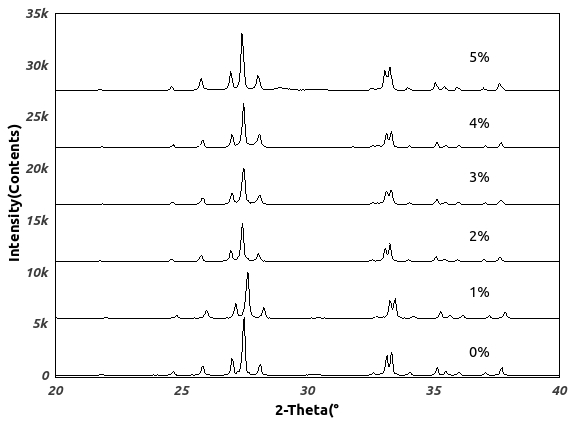
\includegraphics[scale=7]{figures/镨掺杂XRD.jpg} 
\end{block}
\end{frame}

\begin{frame}
\frametitle{镨掺杂系列晶粒尺寸}
\begin{block}{}
\centering
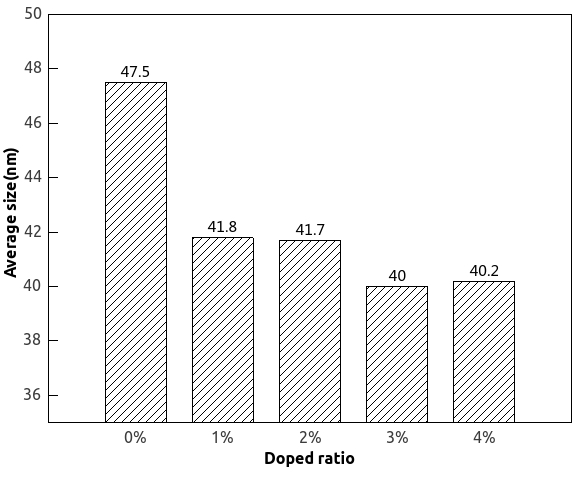
\includegraphics[scale=6]{figures/镨掺杂粒径大小.jpg} 
\end{block}
\end{frame}


\begin{frame}
\frametitle{镨掺杂系列Uv-Vis图谱}
\begin{block}{}
\centering
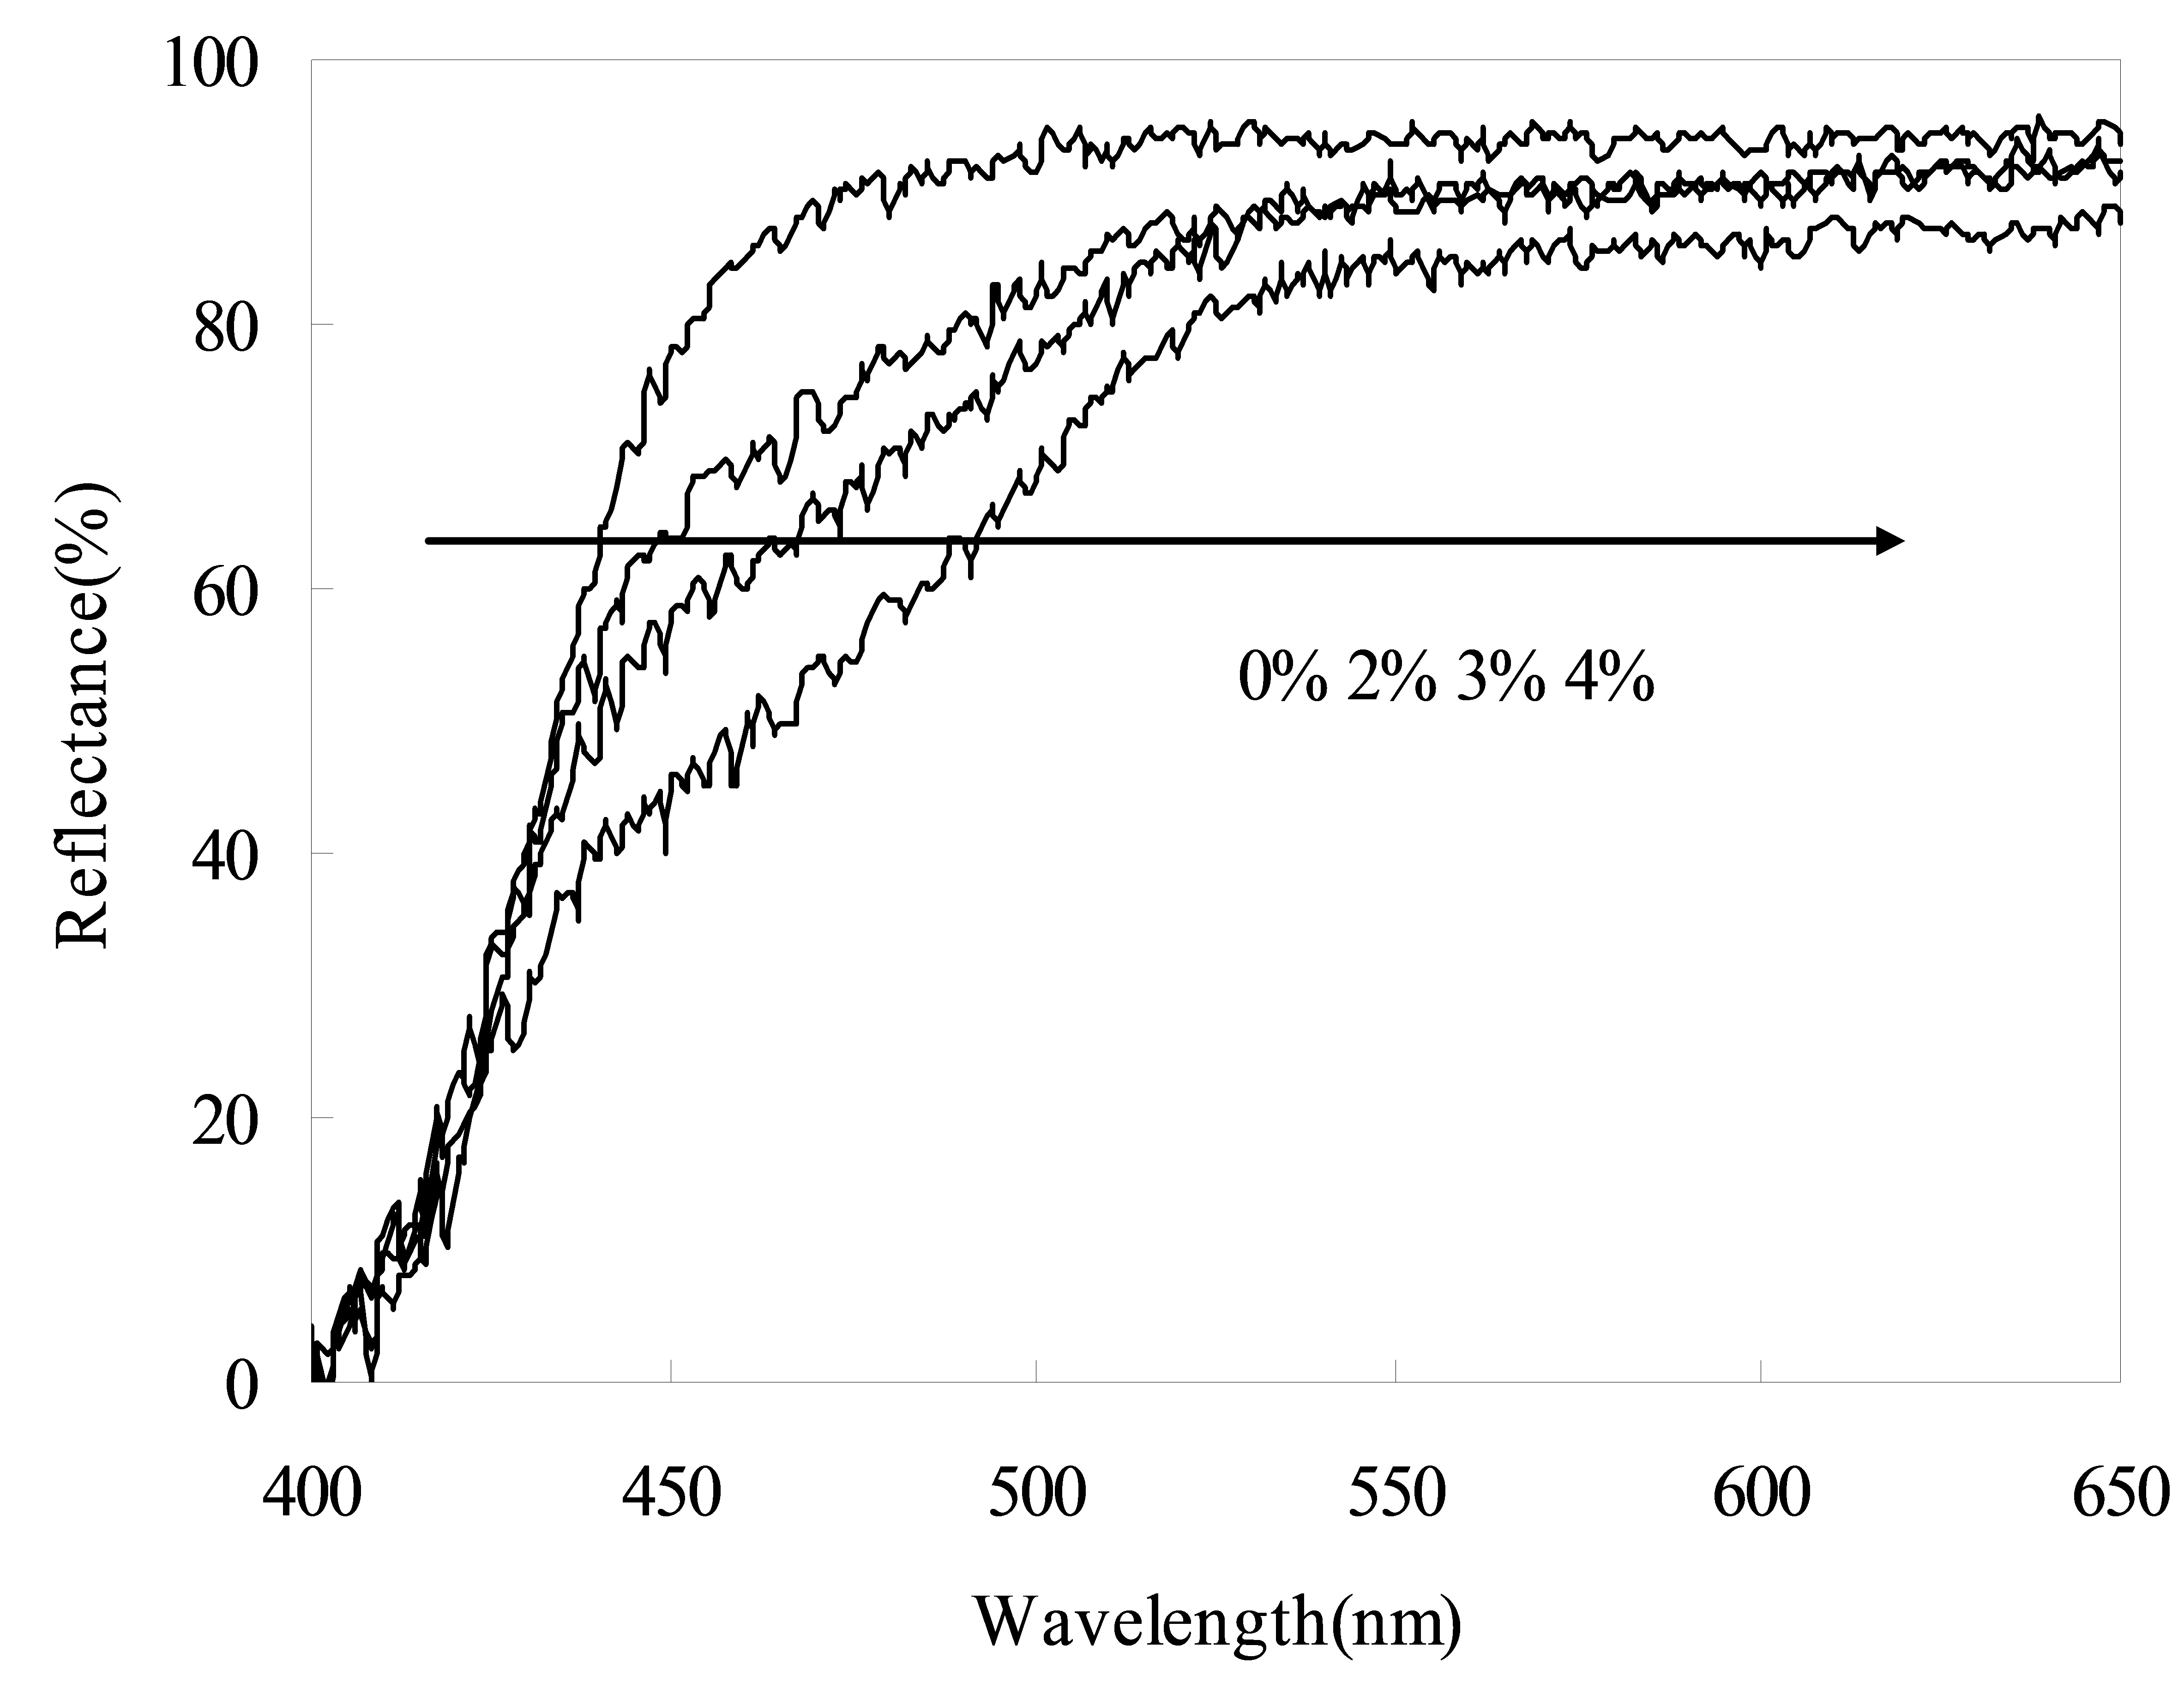
\includegraphics[width=0.8\textwidth]{figures/镨掺杂UV.jpg} 
\end{block}
\end{frame}


\begin{frame}
\frametitle{镨掺杂系列SPS图谱}
\begin{block}{}
\centering
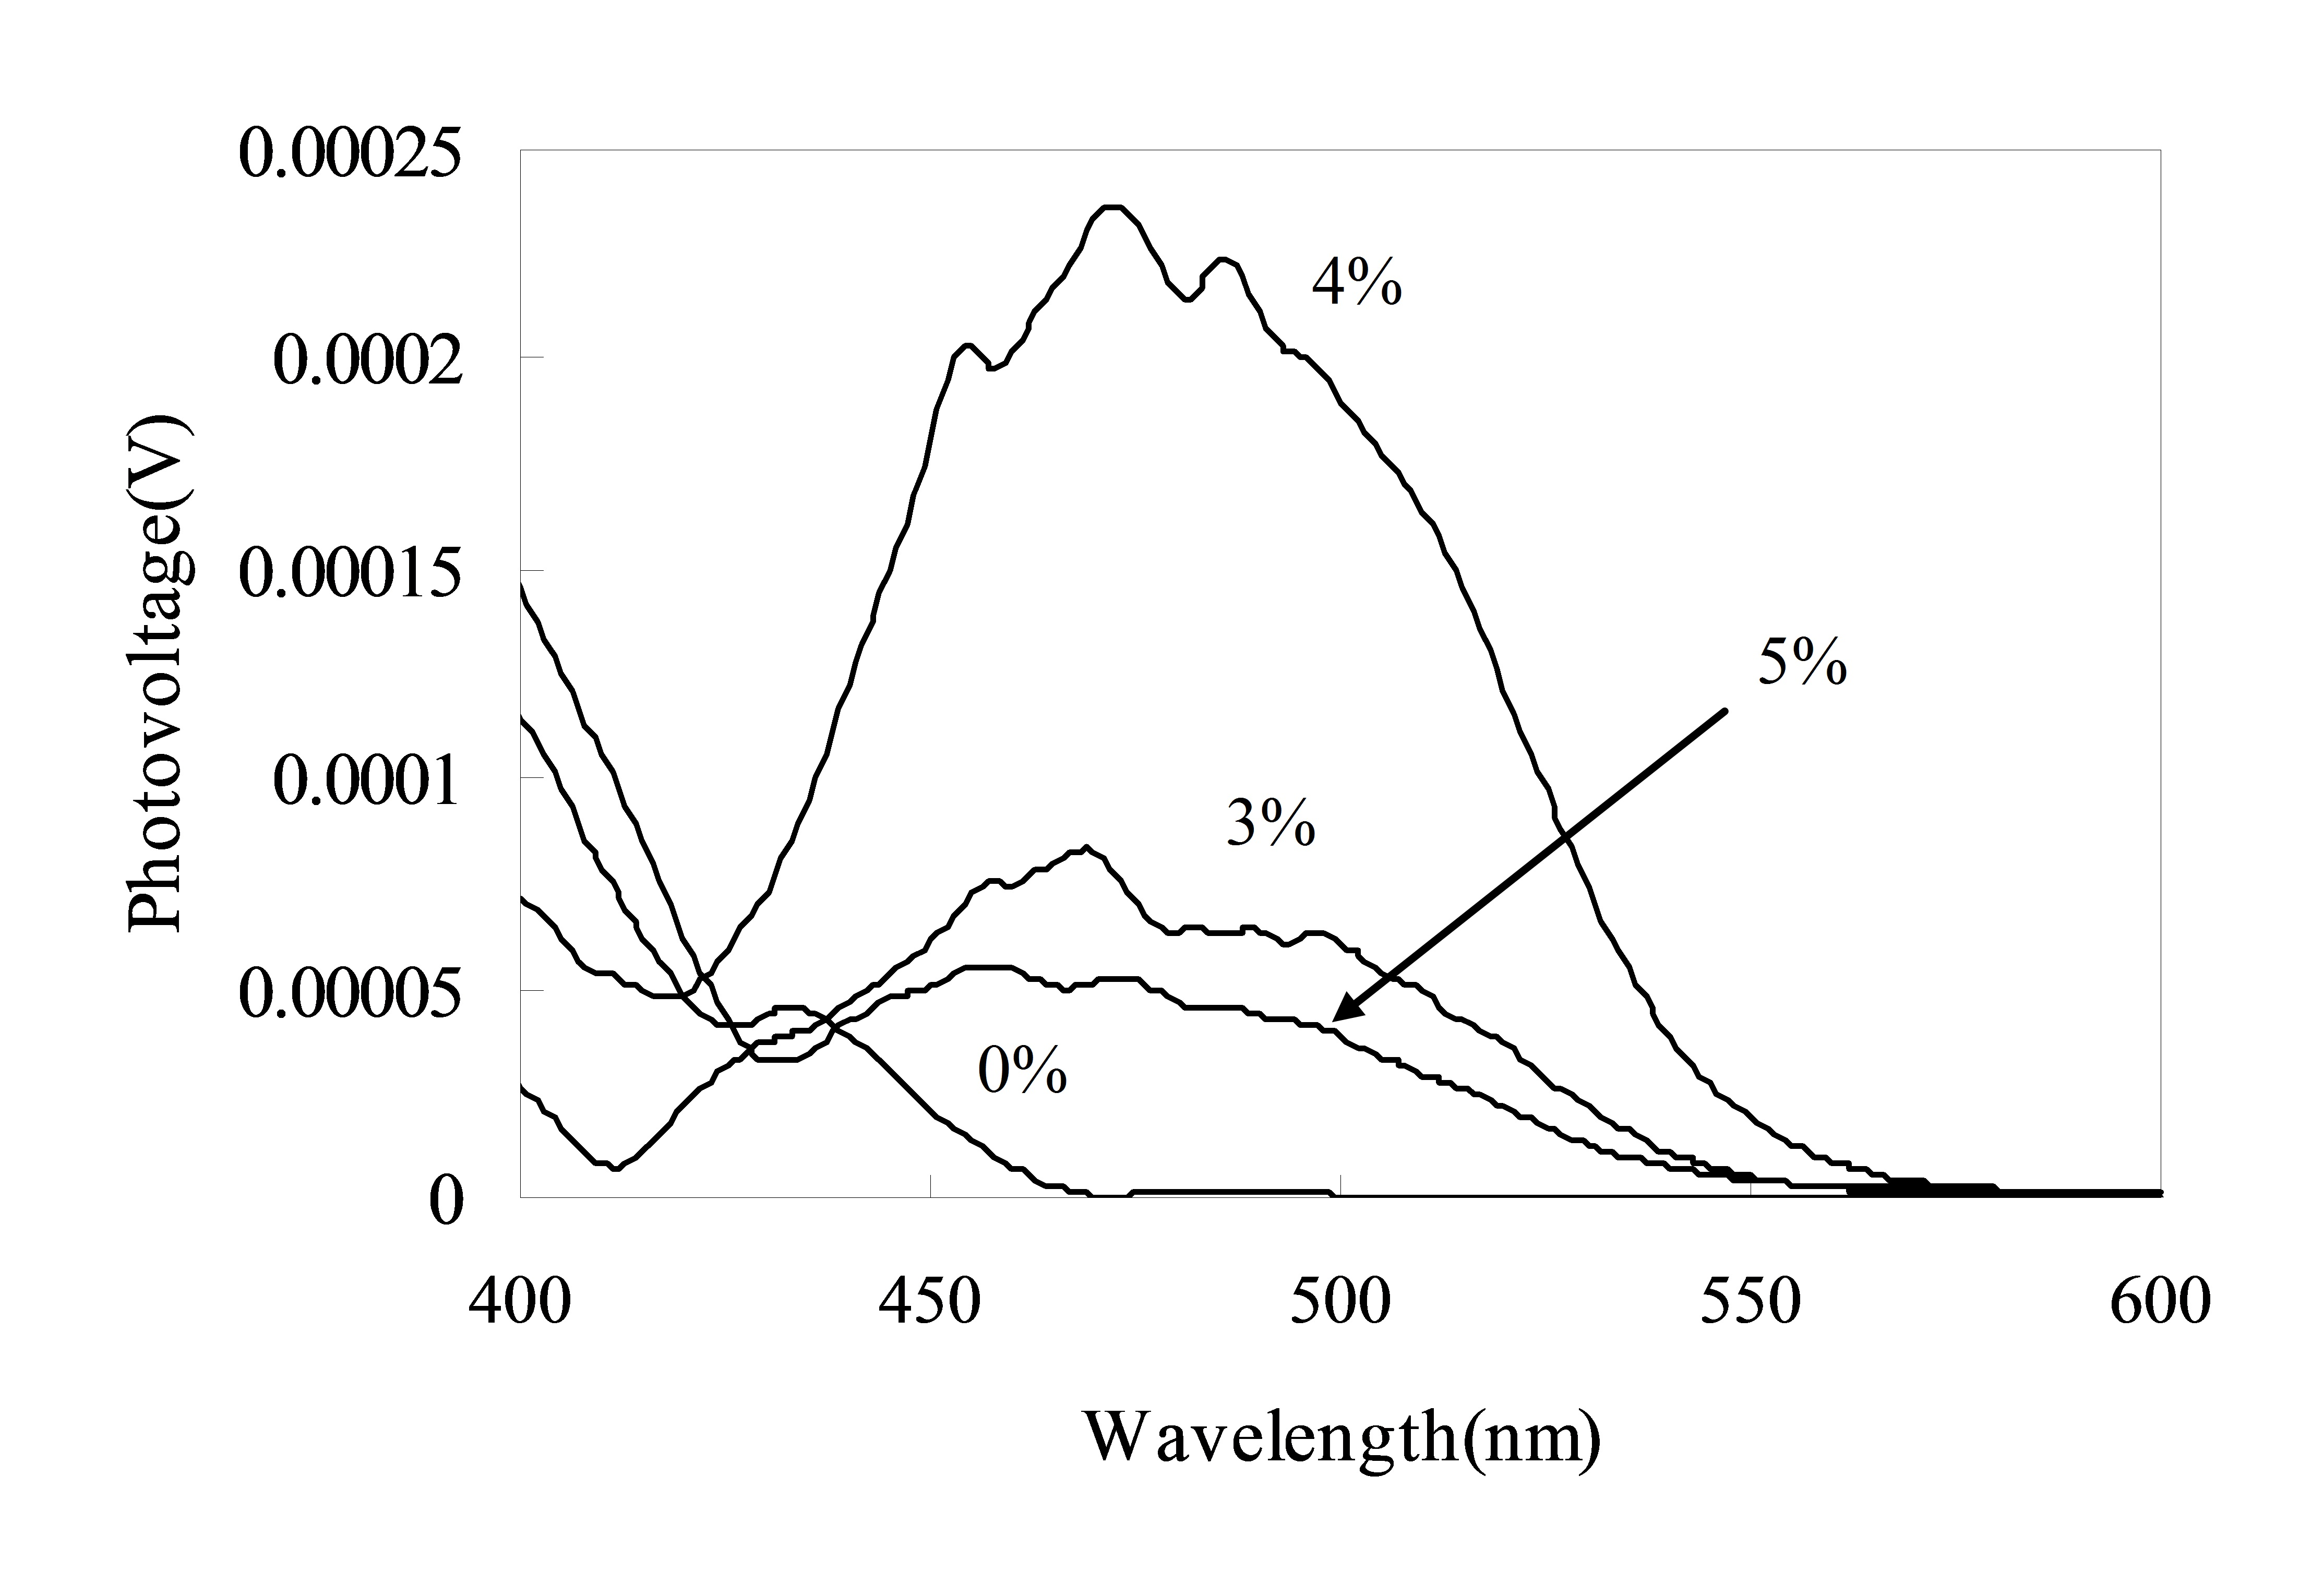
\includegraphics[width=0.8\textwidth]{figures/镨掺杂SPS.jpg} 
\end{block}
\end{frame}


\begin{frame}
\frametitle{镨掺杂系列的光催化活性一}
\framesubtitle{在35W紫外杀菌灯下照射1h}
\begin{block}{}
\centering
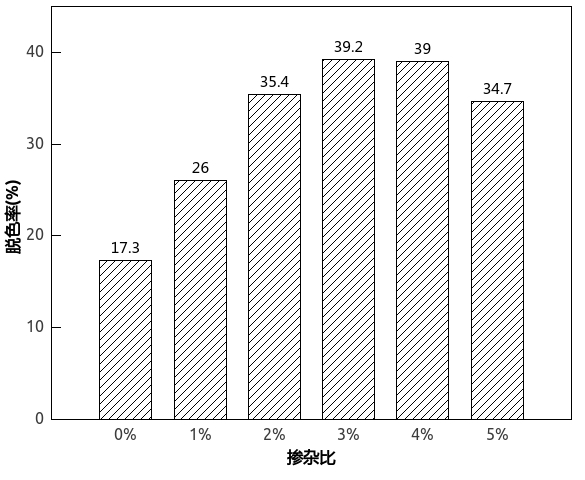
\includegraphics[scale=6]{figures/镨掺杂活性1.jpg} 
\end{block}
\end{frame}

\begin{frame}
\frametitle{镨掺杂系列的光催化活性二}
\framesubtitle{在350W氙灯下照射4h}
\begin{block}{}
\centering
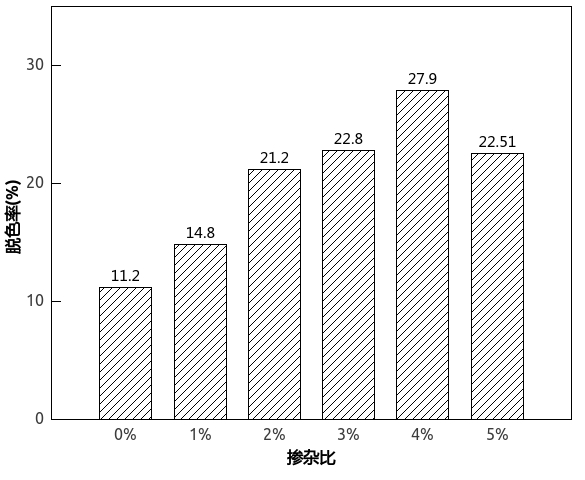
\includegraphics[scale=6]{figures/镨掺杂活性2.jpg} 
\end{block}
\end{frame}


\subsection{钕掺杂}
\begin{frame}
\frametitle{钕掺杂系列XRD图谱}
\begin{block}{}
\centering
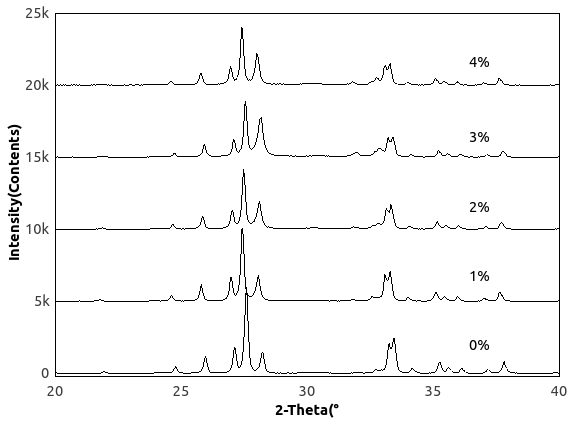
\includegraphics[scale=7]{figures/钕掺杂XRD.jpg} 
\end{block}
\end{frame}

\begin{frame}
\frametitle{钕掺杂系列晶粒尺寸}
\begin{block}{}
\centering
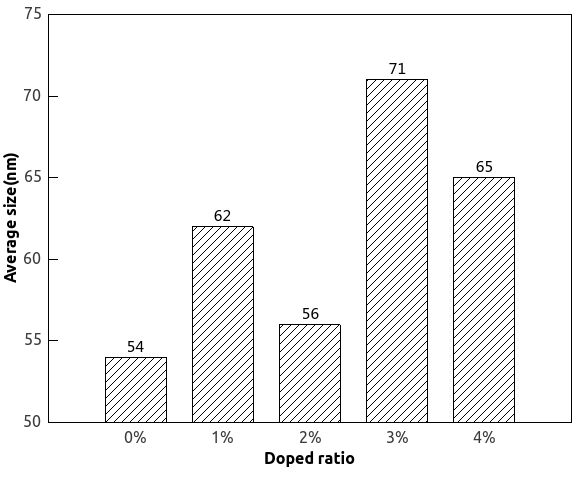
\includegraphics[scale=6]{figures/钕掺杂粒径大小.jpg} 
\end{block}
\end{frame}


\begin{frame}
\frametitle{钕掺杂系列Uv-Vis图谱}
\begin{block}{}
\centering
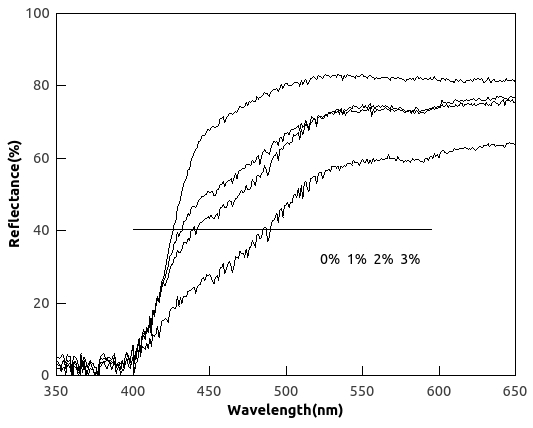
\includegraphics[scale=7]{figures/钕掺杂UV.jpg} 
\end{block}
\end{frame}



\begin{frame}
\frametitle{钕掺杂系列SPS图谱}
\begin{block}{}
\centering
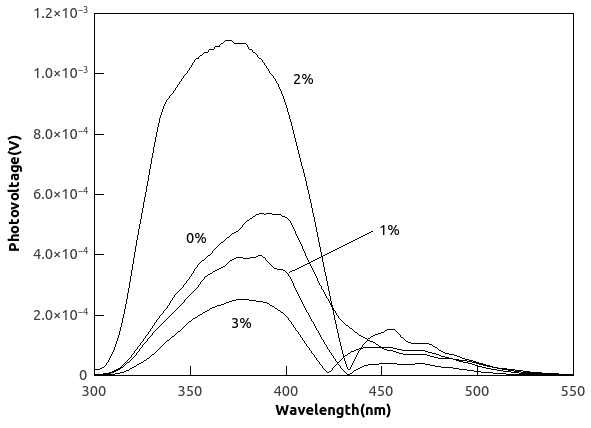
\includegraphics[scale=7]{figures/钕掺杂SPS.jpg} 
\end{block}
\end{frame}


\begin{frame}
\frametitle{钕掺杂系列的光催化活性}
\framesubtitle{在350W氙灯下照射4h}
\begin{block}{}
\centering
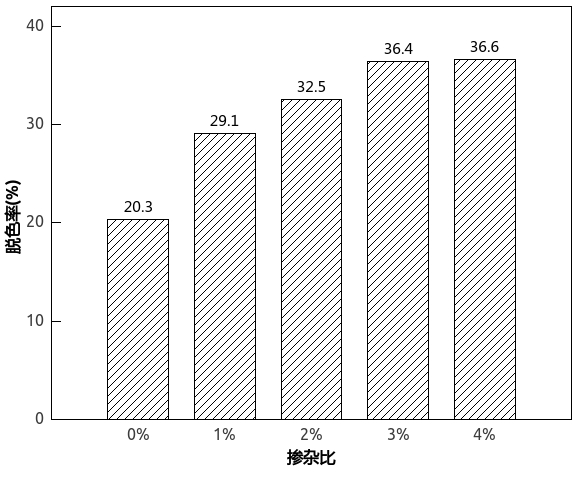
\includegraphics[scale=6]{figures/钕掺杂活性.jpg} 
\end{block}
\end{frame}

\subsection{掺杂改性总结}
\begin{frame}
\frametitle{掺杂改性总结}
\begin{block}{}
\begin{itemize}
\item<1> 掺杂Pr3+后Bi2O3晶粒尺寸变小,比表面增加,对可见光的响应增强,4\%掺杂量样品在可见光区表面光电压响应最强,在模拟太阳光和紫外光照射下掺杂样品对甲基橙光催化活性得到显著提高,其中4\%Pr掺杂样品具有最好的可见光催化活性。%\pause
\item<2> 掺杂Nd3+后Bi2O3晶粒尺寸变大,对可见光的响应增强,2\%掺杂量样品在可见光区表面光电压响应最强,在模拟太阳光照射下对甲基橙光催化活性得到显著提高,其中3\%-4\%Nd掺杂样品具有最好的可见光催化活性。
\end{itemize}
\end{block}
\end{frame}


\section{异质结改性的研究}
\subsection{三氧化二铟}
\begin{frame}
\frametitle{In2O3/ Bi2O3异质结的制备}

\end{frame}


\subsection{三氧化二铁}

\subsection{氧化镍}

\subsection{氧化锌}

%<1>  first show <2> second show [<+->]依次显示 <1-2>1,2都显示 <1->从1一直显示
\begin{frame}
\frametitle{异质结改性总结一}
\begin{block}{}
\begin{itemize}
\item<1> 在Bi2O3表面负载In2O3后表征结果显示形成了In2O3/Bi2O3异质结,In2O3和 Bi2O3存在强的耦合作用,从而光生载流子分离效应增强,在日光照射下所制备异质结对甲基橙光催化活性得到显著提高,其In/Bi原子比为2\%时样品具有最好的太阳光催化活性。%pause
\item<2> 在Bi2O3表面负载Fe2O3后表征结果显示形成了α-Fe2O3/Bi2O3异质结,部分Fe3+离子进入Bi2O3晶格,引起特征衍射峰的位移,α-Fe2O3和 Bi2O3存在强的耦合作用,从而光生载流子分离效应增强,能带值降低,所制备异质结对甲基橙光催化活性得到显著提高,Fe/Bi原子比为3\%样品具有最好的太阳光和紫外光催化活性。
\end{itemize}
\end{block}
\end{frame}

\begin{frame}
\frametitle{异质结改性总结二}
\begin{block}{}
\begin{itemize}
\item<1> 在Bi2O3表面负载 NiO后比表面增加,NiO和 Bi2O3存在强的耦合作用,异质结在400到800 nm区域内对光有着更好的吸收,Ni/Bi原子比为2\%样品具有紫外光催化活性,光照1小时后2\%样品对甲基橙的脱色率较Bi2O3对甲基橙的脱色率提高了约4倍。%\pause
\item<2> ZnO/Bi2O3 异质结的比表面随着ZnO含量增加而逐渐增加,ZnO和 Bi2O3存在强的耦合作用,光催化活性随ZnO含量增加而提高。
\end{itemize}
\end{block}
\end{frame}



\section{总结}
\begin{frame}
\frametitle{总结}
\end{frame}


\subsection{结论和展望}
\begin{frame}
\frametitle{结论和展望}

\end{frame}

\subsection{创新点}
\begin{frame}
\frametitle{创新点}

\end{frame}


\subsection{下一步工作的展望}
\begin{frame}
\frametitle{下一步工作的展望}

\end{frame}


\subsection{致谢}
\begin{frame}
\frametitle{致谢}

\end{frame}

\end{document}
